\chapter{Referencial teórico}\label{cap:referencialTeorico}

\section{Áudio digital}

\subsection{Amostragem}
Uma amostragem é a representação numérica da amplitude sonora em um certo período de tempo, sendo a menor quantidade utilizável de áudio digital. Uma gravação com taxa de amostragem de 44KHz, por exemplo, implica em 44000 valores amostrados de um sinal original a cada segundo.

\subsection{Teorema de Amostragem}
\color{orange}
Um sinal analógico é infinito

Queremos gravá-lo em uma quantidade finita e de preferência a menor quantidade de dados possível

Como saber qual a quantidade mínima de amostragens necessária para reproduzir o original?

Podemos nos basear na fisiologia humana média para determinarmos qual uma faixa ideal

Humanos conseguem ouvir acima de 20khz, mas o sinal precisa ter uma amplitude enorme para que seja detectável

Não vale a pena o esforço para reproduzirmos essas faixas

Samples: arrays of discrete, evenly time-spaced numbers

\begin{displayquote}
"Seja um sinal, limitado em banda, e seu intervalo de tempo dividido em partes iguais, de forma que se obtenham intervalos tais que, cada subdivisão compreenda um intervalo com período T segundos, onde T é menor do que fm/2, e se uma amostra instantânea é tomada arbitrariamente de cada subintervalo, então o conhecimento da amplitude instantânea de cada amostra somado ao conhecimento dos instantes em que é tomada a amostra de cada subintervalo contém toda a informação do sinal original."
\end{displayquote}

\color{black}


\subsection{Canais de Áudio}
Um canal de áudio é definido como a representação de um som proveniente de um único ponto. Um microfone, por exemplo, pode ser utilizado para produzir um canal de áudio, enquanto uma caixa de som reproduz também um canal de áudio.

Áudio digital pode possuir uma quantidade diversa de canais de dados.

Uma música mixada profissionalmente para fones de ouvido será salvo em um arquivo que possuirá dois canais, com cada um contendo dados que devem ser enviados para cada um dos lados do fone de ouvido. Já áudio mixado para som \textit{surround} no contexto de produção de filmes possuirá tipicamente 6 canais.

% https://caseguard.com/articles/the-various-complexities-of-audio-channels-new-recordings/#:~:text=An%20audio%20channel%20is%20defined,have%20numerous%20channels%20of%20data.
\subsection{Modulação por código de pulsos (PCM)}
A modulação por código de pulsos é utilizada para realizar uma representação digital de um sinal analógico. Essa modulação é feita com a amostragem da amplitude de um sinal em intervalos regulares, onde os valores obtidos são então convertidos em representações binárias para que possam posteriormente ser transmitidos.

Esta conversão é tipicamente realizada com a utilização de um conversor analógico-digital. A quantização de um sinal analógico em intervalos regulares permite com que estes sejam facilmente codificados para posterior armazenamento ou manipulação.

% https://www.techopedia.com/definition/24128/pulse-code-modulation-pcm



% https://www.youtube.com/watch?v=Z0EMObqS90U&list=PLbqhA-NKGP6B6V_AiS-jbvSzdd7nbwwCw&index=3

\subsection{I2S}
O protocolo I2S (Inter-IC Sound) é um protocolo serial utilizado para a conexão de dispositivos de áudio. Criado em 1986 pela Phillips Semiconductors (agora NXP Semiconductors), sua finalidade é a  propagação de áudio PCM entre diferentes circuitos integrados.
O barramento consiste de ao menos três linhas:
\begin{itemize}
    \item SCK (continuous serial clock): pulsa para cada bit nas linhas de dados. Sua frequência é baseada na taxa de amostragem, número de bits por canal e número de canais.
    \item WS (Word Select): Informa qual canal está sendo utilizado. O protocolo I2S permite que dois canais sejam enviados em uma mesma linha de dados. Em uma transmissão stereo, é definido que o canal esquerdo seja transferido quando esta linha estiver em baixa, e o canal direito quando ele estiver em alta. Sua sincronização é tipicamente feita na borda de descida desta linha, já que dados são inseridos na borda de subida.
    % https://web.archive.org/web/20070102004400/http://www.nxp.com/acrobat_download/various/I2SBUS.pdf
    \item SD (Serial Data): Linha onde são enviados os dados. Dados são enviados com sinal, codificados em complemento de dois, com o bit mais significativo por primeiro. Isso permite que o número de bits por quadro seja arbitrário, sem necessidade de negociação entre o transmissor e o receptor.
\end{itemize}
\begin{figure}[!h]F
    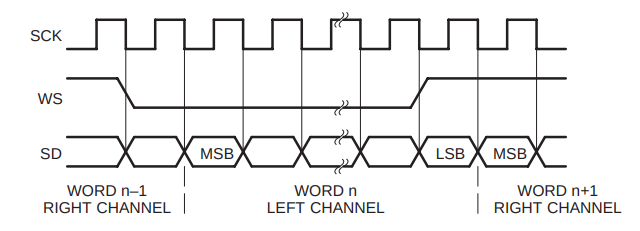
\includegraphics[scale=0.5]{figuras/i2s-bus.png}
    \caption{!! TROCAR POR VERSÃO DE AUTORIA PRÓPRIA !!}
    \label{fig:circularBuffer}
\end{figure}

\section{USB}
O USB (Universal Serial Bus) é um dos padrões da indústria mais utilizadas no mundo. Sua finalidade é a padronização da conexão de dispositivos periféricos à computadores, reduzindo a necessidade de diversas interfaces como portas seriais, paralelas, ADB etc. 
Sua identificação pelo dispositivo receptor é feita por meio de classes USB. Classes podem ser definidas como grupos de dispositivos semelhantes, como de interface humana, armazenamento em massa ou áudio. Ao realizar conexão, o dispositivo é automaticamente identificado e inicializado dependendo do código de classe informado.

Este padrão é também um ótimo candidato para a transmissão de áudio digital, possuindo largura de banda para suficiente para transmissão de áudio de alta qualidade.
Ainda sim, a transmissão e reprodução de áudio por esse protocolo não é uma tarefa simples. Além das complexidades inerentes do próprio protocolo, a transmissão de áudio também traz outro leque de dificuldades, como sincronização, codificação/decodificação e conversão digital-analógica. 

\subsection{Velocidades de transmissão}
A especificação USB 2.0 permite três diferentes velocidades de comunicação: \textit{low speed}, de 1.5 megabits por segundo, \textit{full speed}, de 12 megabits por segundo, e high speed, de 480 megabits por segundo. Um dispositivo \textit{low speed} sempre se conectará  nessa velocidade, independente das capacidades de transmissão do dispositivo \textit{host}. Da mesma forma, um positivo \textit{full speed} sempre se conectará nessa velocidade. Um dispositivo \textit{high speed}, porém, se conecta inicialmente em \textit{full speed}, e tenta uma transição para \textit{full speed} posteriormente, caso o dispositivo \textit{host} seja capaz dessa velocidade.
% https://www.ti.com/video/6305893689112#transcript-tab

\subsection{Transmissão por quadros}
A transmissão de dados de áudio por USB é feita na linha de dados com modulação por pulso de código. O sinal é enviado em quadros, que se refere a uma amostragem de cada canal presente no áudio original.

% https://sound.stackexchange.com/questions/41567/difference-between-frame-and-sample-in-waveform#:~:text=A%20sample%20is%20the%20smallest,during%20a%20video%20frame%20interval.

\subsection{Classe de Interface de Áudio USB}

A classe de interface de áudio agrupa qualquer aplicação que possa interagir com transferências de dados de áudio USB.
Entre as aplicações que se encaixam nesse quesito estão aplicações que convertem entre os domínios analógico e digital, e aplicações que transformem uma transferência de dados em outra transferência também compatível com USB. Mesmo aplicações que interajam diretamente com áudio analógico, porém sejam controladas por USB podem se encaixar nessa classe.

O único requisito obrigatório para uma aplicação ser reconhecida como um dispositivo de interface de áudio é expor uma interface de controle de áudio. Porém, para possibilitar um maior leque de funcionalidades, as aplicações muitas vezes também implementam interfaces de transferência de áudio, para o consumo ou produção de dados.

Audio Interface Class Code

\begin{table}[h]
\begin{tabular}{|l|l|}
\hline
Código & Valor \\ \hline
AUDIO  & 0x01  \\ \hline
\end{tabular}
\caption{Lista de códigos de classe de interface de áudio}
\label{tab:codigos-interface-audio}
\end{table}

\begin{table}[h]
\begin{tabular}{|l|l|}
\hline
Subcódigo           & Valor \\ \hline
SUBCLASS\_UNDEFINED & 0x00  \\ \hline
AUDIOCONTROL        & 0x01  \\ \hline
AUDIOSTREAMING      & 0x02  \\ \hline
MIDISTREAMING       & 0x03  \\ \hline
\end{tabular}
\caption{Lista de subcódigos de classe de interface de áudio}
\label{tab:subcodigos-interface-audio}
\end{table}
\subsection{Padrão USB Audio 1.0}


Para que a propagação e controle do sinal digital de áudio seja feita de maneira que mantenha a interoperabilidade (que é um dos principais fatores de adoção do protocolo USB, a organização USB desenvolveu a definição para dispositivos de áudio (\textit{Universal Serial Bus Device Class Definition for Audio Devices}).
% https://www.mouser.com/pdfDocs/usb-audio-simplified.pdf

Proposto em 1999, este padrão tem seu nome devido a ser feito em cima do padrão USB 1.0 e descreve algumas especificações necessárias para que dispositivos possam ser considerados capazes de reprodução de áudio por USB.


Essa definição é pública, e define características que os dispositivos de áudio devem possuir, como devem se comportar, quais agentes descritores devem estar presentes, entre outros fatores. 

Um dos maiores problemas com a transmissão de áudio via USB é a sincronização do fluxo de dados entre o dispositivo realizando o envio (chamado de \textit{source}), e o receptor (chamado de \textit{sink}). 

Um mecanismo de sincronização chamado de \textit{transferência isosíncrona} foi então desenvolvido e incorporado nessa especificação, no intuito de mitigar essa dificuldade. Devido à isso, implementações comumente requerem sistemas embarcados complexos para conversão de dados e \textit{Phase Locked Loops (PLLs)} para que a precisão necessária de \textit{clock} seja obtida. 

A transmissão isócrona é unidirecional e contínua, e possui um foco maior no \textit{timing} do que na precisão dos dados entregues. Cada frame é reservado com o mesmo tamanho e entregue dentro de um latência estimada. Não há uso de buffers ou correção de erros nesse formato, fazendo com que caso um dado entregue não seja consumido dentro do tempo esperado, ele será perdido. 
% https://www.jungo.com/st/support/documentation/windriver/10.2.1/wdusb_manual.mhtml/USB_data_transfer_types.html

Este formato de transmissão também pode ser subdividido em três tipos de operações: assíncrona, síncrona e adaptável.

No sub-modo assíncrono, o receptor fornece feedback para a fonte. Baseado nesse feedback, a fonte ajusta o número de \textit{samples} que devem ser enviados para o receptor.

No sub-modo síncrono, a fonte e o receptor utilizam feedback implícito, baseado no SOF (Start of Frame) do USB. Ambos precisam se sincronizar com o SOF.
% https://www.mouser.com/pdfDocs/usb-audio-simplified.pdf

Por fim, o sub-modo adaptativo, o receptor se adapta à taxa potencialmente variante do transmissor. 



\begin{figure}[!h]
  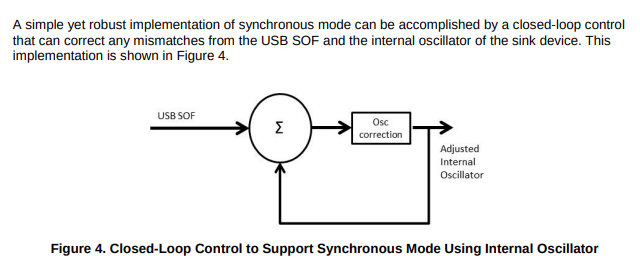
\includegraphics[scale=0.5]{figuras/synchronousmode.png}
  \caption{!! TROCAR POR VERSÃO DE AUTORIA PRÓPRIA !!}
  \label{fig:synchronousMode}
\end{figure}


% https://www.mouser.com/pdfDocs/usb-audio-simplified.pdf 

% [https://www.keil.com/pack/doc/mw/USB/html/_u_s_b__isochronous__transfers.html#:~:text=Isochronous Transfers are used for,delivered at the desired rate](https://www.keil.com/pack/doc/mw/USB/html/_u_s_b__isochronous__transfers.html#:~:text=Isochronous%20Transfers%20are%20used%20for,delivered%20at%20the%20desired%20rate).

% https://docs.teradici.com/knowledge/what-are-usb-transfer-types

% http://www.on-time.com/rtos-32-docs/rtusb-32/programming-manual/advanced-topics/isochronous.htm

A implementação de \textit{drivers} para essa classe de dispositivos permite que o sistema operacional reconheça o dispositivo e possa utilizá-lo para entrada e saída de áudio. 

Para garantir a interoperabilidade entre sistemas e manter os \textit{drivers} o mais genérico possíveis, os mecanismos de conectividade e transporte de dados de áudio precisam ser muito bem definidos e padronizados.  Padrões como a classe de áudio USB 1.0, detalhada adiante, procuram trazer uma solução para esta questão.





No USB Full Speed, um frame se refere a uma transferência de 1ms de duração, com tamanho de 1023 bytes (possuindo assim uma taxa de transferência máxima de 1023kb/s).

% https://microchipdeveloper.com/usb:frames
% https://www.beyondlogic.org/usbnutshell/usb4.shtml



\section{Processamento Digital de Áudio}
Processamento digital de áudio se refere a uma seção do processamento de sinais com foco na manipulação de sinais de áudio, sendo esses representações digitais de ondas sonoras.
Seu uso inicial era focado em invenções como o telefone e o rádio, que necessitavam de manipulação para vencer problemas inerentes da tecnologia, relacionados a sua transmissão.
Após avanços na teoria da comunicação, do teorema da amostragem e da invenção da modulação por código de pulso, um novo leque de aplicações se mostrou possível, inclusive na área de manipulação e até criação de música.
Hoje, métodos de processamento abrangem desde armazenamento e compressão até síntese e melhorias, como equalização, filtragem, compressão e redução ativa de ruído. Essas melhorias são utilizadas com focos para consumidores finais ou em âmbitos profissionais. Em exemplo, o cancelamento de ruído é utilizado em fones de ouvido comuns para remoção de ruídos como transporte, e aplicado em ambientes profissionais que requerem um nivel acima de cancelamento do atingido por métodos passivos).

\subsection{Filtros FIR/IIR}

Filtros digitais são divididos em duas categorias: filtros de resposta de impulso infinita (Infinite Impulse Response, IIR) e resposta de impulso finita (Finite Impulse Response, FIR). 
A distinção entreo os dois se dá devido à sua capacidade ou não de gerar um uma resposta infinita a partir de um sinal finito. A diferença principal consta em sua recursividade, sendo os filtros de resposta de impulso infinita recursivos, e os de resposta de impulso finita não-recursivos.


Filtros de resposta de impulso infinita tendem a ser preferíveis para processamento digital de áudio, devido a sua eficiência computacional. Enquanto filtros de resposta de impulso finita utilizam uma implementação convolucional, a possibilidade de utilização de retroalimentação em filtros de resposta de impulso infinita facilita sua implementação, dependendo apenas de somas e multiplicações de valores anteriores em memória.

Filtros de resposta finita precisam de mais coeficientes para atingirem um \textit{rolloff} esperado, e quanto mais termos são adicionados, maior será o atraso adicionado à saída.
Filtros de resposta infinita, embora tenham que lidar com possíveis problemas de estabilidade, conseguem entregar um \textit{rolloff} em menos termos e adicionando pouco atraso à saída. Como aplicações de áudio USB podem necessitar de respostas em quase tempo real, como telecomunicações, idealmente deve ser adicionado o mínimo de atraso possível ao sinal original.
% https://www.collimator.ai/reference-guides/what-is-an-fir-vs-iir-filter
% https://www.juansaudio.com/post/iir-vs-fir-understanding-their-differences
% https://www.advsolned.com/difference-between-iir-and-fir-filters-a-practical-design-guide/
% https://community.sw.siemens.com/s/article/introduction-to-filters-fir-versus-iir
\subsection{Filtros discretos}
\subsection{Filtros de Equalização (Passa-faixas)}

% Uma forma de tratar o referencial teórico é definir como título de capítulo o assunto macro e relevante relacionado ao trabalho e o texto é dividido em subtítulos (seções e subseções), conforme necessário. Essa forma é preferida por deixar explícito o assunto a ser tratado e que o mesmo é a fundamentação do trabalho \footnote{Teste de nota de rodapé 3.}. 

% Outra forma de tratar esse capítulo é denominá-lo referencial teórico e dividi-lo em seções e subseções ou com um único texto os assuntos que fornecem o suporte teórico para o trabalho. Essa forma pode ser utilizada quando assuntos distintos fundamentam o trabalho e é difícil incluí-los sob uma mesma denominação de capítulo \footnote{Teste de nota de rodapé 4.}.

% O embasamento teórico se refere ao(s) assunto(s) principal(is) relacionado(s) ao objeto de pesquisa para o qual o trabalho traz alguma contribuição ou que é utilizado como referência conceitual para o desenvolvimento do proposto no trabalho. O assunto pode fornecer a fundamentação (suporte teórico) para a ideia do sistema, para definir claramente o problema, para explicitar a solução, para a forma de resolução; referir-se aos conceitos e teorias relacionados ao sistema desenvolvido, sobre tecnologias e metodologias específicas utilizadas na definição do sistema e na sua implementação.

% Exemplos:

% Conceitos da orientação a objetos fazem parte do referencial teórico se o uso intensivo da orientação a objetos é o principal embasamento do trabalho; ou se a principal contribuição do trabalho está relacionada à orientação a objetos, seja em termos de agregar conhecimento nessa área ou à forma de usar os seus conceitos.

% Sistemas distribuídos pode ser o assunto do embasamento teórico se o resultado do trabalho for um sistema distribuído. O mesmo pode ocorrer com sistemas cliente servidor, sistemas de informações gerenciais, de apoio à decisão, para web e etc.

% Se o desenvolvimento de um sistema para biometria for o objeto do trabalho, o referencial teórico se refere aos conceitos principais de biometria, aplicabilidade, exemplos de sistemas existentes, o que esses sistemas tratam, como eles são, etc.

% Se um sistema web para portadores de necessidades especiais for o resultado do trabalho, o referencial teórico refere-se as quais e como são essas necessidades, outros sistemas existentes na área, como os sistemas lidam com essas necessidades e os principais conceitos por eles considerados.

% O embasamento teórico pode conter os trabalhos relacionados, desde que seja relevante para o desenvolvimento do trabalho. Esse item deve ser elaborado especialmente quando se trata do desenvolvimento de algo muito específico, havendo a necessidade de um estudo comparativo. Nesse caso pode-se inserir claramente o trabalho de pesquisa no contexto dos demais autores, no sentido da contribuição da proposta na área de pesquisa em que o mesmo se insere e em relação ao que já tem pesquisado na área. 

% \caixa{Atenção}{Converse com o seu orientador para ver quais seções/conteúdos devem ter neste capítulo...}

% \section{Observações sobre a citações}\label{sec:formatacaoTexto}

% O texto em si é dividido em títulos e subtítulos, se necessário. 

% O espaçamento entre linhas é de 1,5. Os títulos das seções primárias e das demais subseções devem ser separados do texto que os precede ou que os sucede por uma linha em branco. As seções primárias devem iniciar em páginas distintas.

% Com relação à paginação, todas as folhas do trabalho, a partir da folha de rosto, devem ser contadas sequencialmente, mas não numeradas. A numeração deve ser colocada a partir da primeira folha da parte textual (introdução), em algarismos arábicos, no canto superior direito da folha.

% \caixa{Observação}{Se você estiver utilizando \latex, não é necessário se preocupar com formatação.}

% As próximas seções comentam a respeito de citações.

% \subsection{Citações}\label{subsec:citacoes}

% \textbf{Citação direta:} É quando o texto utilizado é transcrito com as próprias palavras do autor. Quando curtas (até três linhas) a transcrição literal virá entre “aspas” e a referência pode ser incluída no texto junto à sentença ou frase, ou ainda ser colocada entre parênteses. Quando inclusa no texto, deve-se usar letras maiúsculas e minúsculas, com indicação da data e demais informações entre parênteses.

% Exemplo de citação direta curta com autor incluso no texto: Segundo \citeonline[p. 107]{Pressman2009} o valor da informação está “diretamente ligado à maneira como ela ajuda os tomadores de decisões a atingirem as metas da organização”. Exemplo de citação direta curta com autor não incluso no texto: O autor lembra, contudo, a análise precursora de \citeonline{Pressman2009} sobre alguns aspectos limitantes das competências, ou aptidões, essenciais, que as transformam em “limitações estratégicas” \cite{Pressman2009}.

% As transcrições com mais de três linhas (citações diretas longas) aparecem recuadas em 4 cm, a partir da margem esquerda, em espaço simples, tamanho 10, e a indicação da fonte é apresentada entre parênteses. 

% \begin{citacao}
% Na nova sociedade, chamada de capitalista: O recurso econômico básico – ‘os meios de produção’, para usar uma expressão dos economistas – não é mais o capital, nem os recursos naturais (a ‘terra’ dos economistas), nem a ‘mão-de-obra’. Ele será o conhecimento. As atividades centrais de criação de riqueza não serão nem a alocação de capital para usos produtivos, nem a ‘mão-de-obra’ – os dois pólos da teoria econômica dos séculos dezenove e vinte, quer ela seja clássica, marxista, keynesiana ou neoclássica. Hoje o valor é criado pela ‘produtividade’ e pela ‘inovação’, que são aplicações do conhecimento ao trabalho. Os principais grupos sociais da sociedade do conhecimento serão os ‘trabalhadores do conhecimento’ – executivos que sabem como alocar conhecimento para usos produtivos. \cite[p. 48]{Pressman2009}.
% \end{citacao}

% \textbf{Citação indireta:} É a reprodução de ideias do autor. É uma citação livre, usando as palavras de quem está escrevendo para dizer o mesmo que o autor disse no texto. Contudo, a ideia expressa continua sendo de autoria do autor consultado, por isso é necessário citar a fonte: dar crédito ao autor da ideia. Exemplo de citação indireta: O valor da informação está relacionado com o poder de ajuda aos tomadores de decisões a atingirem os objetivos da empresa\cite{Pressman2009}. Outra forma de citação indireta: \citeonline{Pressman2009} destacam ser fundamental a gestão de dados nas organizações, pois isso garantirá o funcionamento normal dos sistemas de informação, uma vez que, sem a capacidade de seu processamento, haveria problemas para a empresa executar suas atividades efetivamente.

% Citações de obras que contenham até três autores, devem apresentar os sobrenomes destes separados por ponto e vírgula, como no exemplo: \cite[p. 2]{Pinto2000}. E para obras que contenham mais de três autores indica-se citar apenas o nome do primeiro autor, seguido da expressão abreviada \textit{et al.}, como no exemplo: \cite{Guimaraes2003}.

% \subsection{Ilustrações, quadros e tabelas}\label{subsec:ilustracoes}

% As ilustrações, quadros e tabelas devem aparecer no texto, segundo a NBR14724:2011, de forma padronizada.

% Qualquer que seja o tipo de ilustração, sua identificação aparece na parte superior, precedida da palavra designativa (desenho, esquema, fluxograma, fotografia, gráfico, mapa, organograma, planta, quadro, retrato, figura, imagem, entre outros), seguida de seu número de ordem de ocorrência no texto, em algarismos arábicos, travessão e do respectivo título. Após a ilustração, na parte inferior, indicar a fonte consultada (elemento obrigatório, mesmo que seja produção do próprio autor), legenda, notas e outras informações necessárias à sua compreensão (se houver). A ilustração deve ser citada no texto e inserida o mais próximo possível do trecho a que se refere.

% A fonte, ou seja, a indicação do autor da ilustração ou da publicação de onde ela foi retirada deve aparecer na parte inferior. Exemplo:

% Fonte: \citeonline{Coulouris2013}. 			- quando utilizado o item original

% Fonte: Adaptado de \citeonline{Coulouris2013}.	- quando o item original foi alterado

% Para facilitar a inclusão de fontes, o \textit{template} em LaTeX da \gls{utfpr}, possui o comando \texttt{$\backslash$fonte\{\}}. Se este comando for deixado em branco (\texttt{$\backslash$fonte\{\}}),  ele preencherá automaticamente a fonte com o texto  ``Fonte: Autoria própria (ANO)'', sendo ANO substituído pelo ano atual. Já se o comando \texttt{$\backslash$fonte\{\}} tiver algum conteúdo (não estiver em branco), tal conteúdo será inserido na legenda da fonte e esse conteúdo pode ser uma citação. Por exemplo, o comando \texttt{$\backslash$fonte\{$\backslash$citeonline\{Coulouris2013\}\}} gerará o texto ``Fonte: \citeonline{Coulouris2013}.''. Atenção, não é necessário incluir o ponto final (``.''), no texto do comando \texttt{$\backslash$fonte\{\}}, pois isso é feito automaticamente.  

% A figura também deve ser citada no texto. Primeira opção, como pode ser observado na \autoref{fig:exemplo1}. Segunda opção, como pode ser observado na Figura \ref{fig:exemplo1}.

% \begin{figure}[htb]%% Ambiente figure
%     %\captionsetup{width=0.55\textwidth}%% Largura da legenda
%     \caption{Exemplo de figura criada a partir de um arquivo}%% Legenda
%     \label{fig:exemplo1}%% Rótulo
%     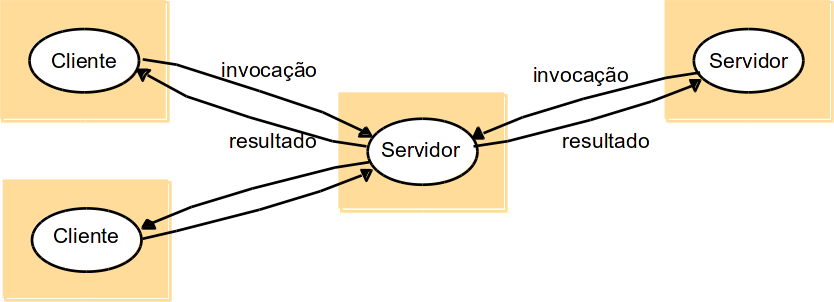
\includegraphics[scale=0.4]{cs2}%% Dimensões e localização
%     \fonte{Adaptado de \citeonline{Coulouris2013}}%% Fonte
% \end{figure}

% Utilizando o pacote \textit{subfig} é possível adicionar figuras lado a lado, como pode ser observado na \autoref{fig:exemplo2}.

% \begin{figure}[htb]
%     \caption{Telas de cadastro de Paciente: (a) Cadastro Paciente, (b) Cadastro Paciente 2} 
% 	\label{fig:exemplo2}
% 	\centering
% 	\subfloat[Cadastro Paciente]{
% 		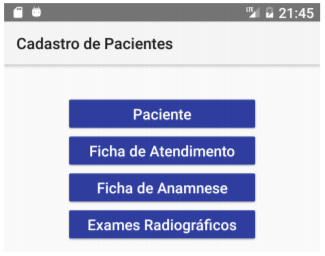
\includegraphics[scale=0.7]{cadastro-paciente}
% 	}\hspace{0.15cm} 
% 	\subfloat[Cadastro Paciente 2]{
% 		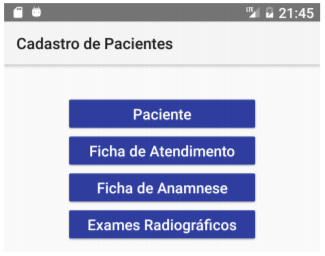
\includegraphics[scale=0.7]{cadastro-paciente}
% 	}
	
% 	\fonte{}
% \end{figure}

% Este modelo vem com o ambiente \texttt{quadro} e impressão de Lista de quadros 
% configurados por padrão.  Este parágrafo apresenta como referenciar o quadro no texto, requisito obrigatório da ABNT. Primeira opção, utilizando \texttt{autoref}: Ver o \autoref{quad:exemplo1}. Segunda opção, utilizando  \texttt{ref}: Ver o Quadro \ref{quad:exemplo1}.

% \begin{tabframed}[htb]%% Ambiente tabframed
% %\captionsetup{width=0.5\textwidth}%% Largura da legenda
% \caption{Materiais utilizados no desenvolvimento do sistema}%% Legenda
% \label{quad:exemplo1}%% Rótulo
% \renewcommand{\arraystretch}{1.5}
% \begin{tabular}{|l|l|l|l|l}
% \cline{1-4}
% \textbf{Ferramenta/Tecnologia} & \textbf{Versão} & \textbf{Disponível em} & \textbf{Finalidade} \\ \cline{1-4}
%  Teste & 1.0  & https:/teste.org & Biblioteca de Teste & \\ \cline{1-4}  
%  Teste & 1.0  & https:/teste.org & Biblioteca de Teste & \\ \cline{1-4}
%  Teste & 1.0  & https:/teste.org & Biblioteca de Teste & \\ \cline{1-4}
%  Teste & 1.0  & https:/teste.org & Biblioteca de Teste & \\ \cline{1-4}
% \end{tabular}
% \fonte{}%% Fonte
% \end{tabframed}


% Também é possível citar tabelas no texto. Primeira opção, utilizando \texttt{autoref}: Ver o \autoref{tab:exemplo1}. Segunda opção, utilizando  \texttt{ref}: Ver a Tabela \ref{tab:exemplo1}.

% \begin{table}[htb]
% % Luiz - O texto do caption da tabela/quadro deve ser do tamanho da tabela, então utilize a linha a seguir para conseguir esse efeito
% \captionsetup{width=0.33\textwidth}
% \centering
% \caption{\label{tab:exemplo1}Exemplo de tabela com uma legenda contendo um texto longo}
% \begin{tabular}{cccc}
% 	\hline
% 	\textbf{Pessoa} & \textbf{Idade} & \textbf{Peso} & \textbf{Altura} \\ \hline
% 	Marcos & 26    & 68   & 178    \\ 
% 	Ivone  & 22    & 57   & 162    \\ 
% 	...    & ...   & ...  & ...    \\ 
% 	Sueli  & 40    & 65   & 153    \\ \hline
% \end{tabular}
% \fonte{}
% \end{table}

% A \autoref{tab:exemplo2} também pode ser citada no texto.

% \begin{table}[htb]%% Ambiente table
% \caption{Segundo exemplo de tabela com uma legenda contendo um texto muito longo que pode ocupar mais de uma linha}%% Legenda
% \label{tab:exemplo2}%% Rótulo
% \begin{tabularx}{\textwidth}{@{\extracolsep{\fill}}llll}%% Ambiente tabularx
% \toprule
% $\bsym{L}$ & $\bsym{L^2}$ & $\bsym{L^3}$ & $\bsym{L^4}$ \\
% \SI{}{[m]} & \SI{}{[m^2]} & \SI{}{[m^3]} & \SI{}{[m^4]} \\ \midrule
% 1          & 1            & 1            & 1            \\
% 2          & 4            & 8            & 16           \\
% 3          & 9            & 27           & 81           \\
% 4          & 16           & 64           & 256          \\
% 5          & 25           & 125          & 625          \\ \bottomrule
% \end{tabularx}
% \fonte{}%% Fonte
% \end{table}

% A \autoref{tab:exemplo3} é um exemplo de tabela que ocupa mais de uma página e que foi construída pelo \gls{latex}\index{LaTeX@\latex} utilizando o pacote \texttt{longtable}.

% \begin{longtable}{@{\extracolsep{\fill}}lll}%% Ambiente longtable
% \caption{Possíveis tríplices para grade altamente variável\label{tab:exemplo3}} \\%% Legenda e rótulo
% \toprule
% \textbf{Tempo (s)} & \textbf{Tríplice escolhida} & \textbf{Outras possíveis tríplices} \\
% \midrule
% \endfirsthead%% Encerra cabeçalho da primeira página
% \caption[]{Possíveis tríplices para grade altamente variável} \\%% Legenda
% \multicolumn{3}{r}{\textbf{(continuação)}} \\
% \toprule
% \textbf{Tempo (s)} & \textbf{Tríplice escolhida} & \textbf{Outras possíveis tríplices} \\
% \midrule
% \endhead%% Encerra cabeçalho das demais páginas
% \midrule
% \multicolumn{3}{r}{\textbf{(continua)}} \\
% \endfoot%% Encerra rodapé das demais páginas
% \bottomrule
% \\[-0.5\linha]
% \caption*{\nomefonte: Adaptado de \citet{Smallen2014}} \\
% \endlastfoot%% Encerra rodapé da última página
% 0      & (1, 11, 13725) & (1, 12, 10980), (1, 13, 8235), (2, 2, 0), (3, 1, 0) \\
% 2745   & (1, 12, 10980) & (1, 13, 8235), (2, 2, 0), (2, 3, 0), (3, 1, 0)      \\
% 5490   & (1, 12, 13725) & (2, 2, 2745), (2, 3, 0), (3, 1, 0)                  \\
% 8235   & (1, 12, 16470) & (1, 13, 13725), (2, 2, 2745), (2, 3, 0), (3, 1, 0)  \\
% 10980  & (1, 12, 16470) & (1, 13, 13725), (2, 2, 2745), (2, 3, 0), (3, 1, 0)  \\
% 13725  & (1, 12, 16470) & (1, 13, 13725), (2, 2, 2745), (2, 3, 0), (3, 1, 0)  \\
% 16470  & (1, 13, 16470) & (2, 2, 2745), (2, 3, 0), (3, 1, 0)                  \\
% 19215  & (1, 12, 16470) & (1, 13, 13725), (2, 2, 2745), (2, 3, 0), (3, 1, 0)  \\
% 21960  & (1, 12, 16470) & (1, 13, 13725), (2, 2, 2745), (2, 3, 0), (3, 1, 0)  \\
% 24705  & (1, 12, 16470) & (1, 13, 13725), (2, 2, 2745), (2, 3, 0), (3, 1, 0)  \\
% 27450  & (1, 12, 16470) & (1, 13, 13725), (2, 2, 2745), (2, 3, 0), (3, 1, 0)  \\
% 30195  & (2, 2, 2745)   & (2, 3, 0), (3, 1, 0)                                \\
% 32940  & (1, 13, 16470) & (2, 2, 2745), (2, 3, 0), (3, 1, 0)                  \\
% 35685  & (1, 13, 13725) & (2, 2, 2745), (2, 3, 0), (3, 1, 0)                  \\
% 38430  & (1, 13, 10980) & (2, 2, 2745), (2, 3, 0), (3, 1, 0)                  \\
% 41175  & (1, 12, 13725) & (1, 13, 10980), (2, 2, 2745), (2, 3, 0), (3, 1, 0)  \\
% 43920  & (1, 13, 10980) & (2, 2, 2745), (2, 3, 0), (3, 1, 0)                  \\
% 46665  & (2, 2, 2745)   & (2, 3, 0), (3, 1, 0)                                \\
% 49410  & (2, 2, 2745)   & (2, 3, 0), (3, 1, 0)                                \\
% 52155  & (1, 12, 16470) & (1, 13, 13725), (2, 2, 2745), (2, 3, 0), (3, 1, 0)  \\
% 54900  & (1, 13, 13725) & (2, 2, 2745), (2, 3, 0), (3, 1, 0)                  \\
% 57645  & (1, 13, 13725) & (2, 2, 2745), (2, 3, 0), (3, 1, 0)                  \\
% 60390  & (1, 12, 13725) & (2, 2, 2745), (2, 3, 0), (3, 1, 0)                  \\
% 63135  & (1, 13, 16470) & (2, 2, 2745), (2, 3, 0), (3, 1, 0)                  \\
% 65880  & (1, 13, 16470) & (2, 2, 2745), (2, 3, 0), (3, 1, 0)                  \\
% 68625  & (2, 2, 2745)   & (2, 3, 0), (3, 1, 0)                                \\
% 71370  & (1, 13, 13725) & (2, 2, 2745), (2, 3, 0), (3, 1, 0)                  \\
% 74115  & (1, 12, 13725) & (2, 2, 2745), (2, 3, 0), (3, 1, 0)                  \\
% 76860  & (1, 13, 13725) & (2, 2, 2745), (2, 3, 0), (3, 1, 0)                  \\
% 79605  & (1, 13, 13725) & (2, 2, 2745), (2, 3, 0), (3, 1, 0)                  \\
% 82350  & (1, 12, 13725) & (2, 2, 2745), (2, 3, 0), (3, 1, 0)                  \\
% 85095  & (1, 12, 13725) & (1, 13, 10980), (2, 2, 2745), (2, 3, 0), (3, 1, 0)  \\
% 87840  & (1, 13, 16470) & (2, 2, 2745), (2, 3, 0), (3, 1, 0)                  \\
% 90585  & (1, 13, 16470) & (2, 2, 2745), (2, 3, 0), (3, 1, 0)                  \\
% 93330  & (1, 13, 13725) & (2, 2, 2745), (2, 3, 0), (3, 1, 0)                  \\
% 96075  & (1, 13, 16470) & (2, 2, 2745), (2, 3, 0), (3, 1, 0)                  \\
% 98820  & (1, 13, 16470) & (2, 2, 2745), (2, 3, 0), (3, 1, 0)                  \\
% 101565 & (1, 13, 13725) & (2, 2, 2745), (2, 3, 0), (3, 1, 0)                  \\
% 104310 & (1, 13, 16470) & (2, 2, 2745), (2, 3, 0), (3, 1, 0)                  \\
% 107055 & (1, 13, 13725) & (2, 2, 2745), (2, 3, 0), (3, 1, 0)                  \\
% 109800 & (1, 13, 13725) & (2, 2, 2745), (2, 3, 0), (3, 1, 0)                  \\
% 112545 & (1, 12, 16470) & (1, 13, 13725), (2, 2, 2745), (2, 3, 0), (3, 1, 0)  \\
% 115290 & (1, 13, 16470) & (2, 2, 2745), (2, 3, 0), (3, 1, 0)                  \\
% 118035 & (1, 13, 13725) & (2, 2, 2745), (2, 3, 0), (3, 1, 0)                  \\
% 120780 & (1, 13, 16470) & (2, 2, 2745), (2, 3, 0), (3, 1, 0)                  \\
% 123525 & (1, 13, 13725) & (2, 2, 2745), (2, 3, 0), (3, 1, 0)                  \\
% 126270 & (1, 12, 16470) & (1, 13, 13725), (2, 2, 2745), (2, 3, 0), (3, 1, 0)  \\
% 129015 & (2, 2, 2745)   & (2, 3, 0), (3, 1, 0)                                \\
% 131760 & (2, 2, 2745)   & (2, 3, 0), (3, 1, 0)                                \\
% 134505 & (1, 13, 16470) & (2, 2, 2745), (2, 3, 0), (3, 1, 0)                  \\
% 137250 & (1, 13, 13725) & (2, 2, 2745), (2, 3, 0), (3, 1, 0)                  \\
% 139995 & (2, 2, 2745)   & (2, 3, 0), (3, 1, 0)                                \\
% 142740 & (2, 2, 2745)   & (2, 3, 0), (3, 1, 0)                                \\
% 145485 & (1, 12, 16470) & (1, 13, 13725), (2, 2, 2745), (2, 3, 0), (3, 1, 0)  \\
% 148230 & (2, 2, 2745)   & (2, 3, 0), (3, 1, 0)                                \\
% 150975 & (1, 13, 16470) & (2, 2, 2745), (2, 3, 0), (3, 1, 0)                  \\
% 153720 & (1, 12, 13725) & (2, 2, 2745), (2, 3, 0), (3, 1, 0)                  \\
% 156465 & (1, 13, 13725) & (2, 2, 2745), (2, 3, 0), (3, 1, 0)                  \\
% 159210 & (1, 13, 13725) & (2, 2, 2745), (2, 3, 0), (3, 1, 0)                  \\
% 161955 & (1, 13, 16470) & (2, 2, 2745), (2, 3, 0), (3, 1, 0)                  \\
% 164700 & (1, 13, 13725) & (2, 2, 2745), (2, 3, 0), (3, 1, 0)                  \\
% \end{longtable}


% \subsection{Códigos fonte e algoritmos}\label{subsec:algoritimos}

% Os algoritmos podem ser utilizados para explicar uma determinada rotina desenvolvida. Conforme pode ser observado no \autoref{alg:exemplo1}.

% \begin{algorithm}[htb]%% Ambiente algorithm
% \caption{Algoritmo de exemplo}%% Legenda
% \label{alg:exemplo1}%% Rótulo
% \hrule
% \begin{algorithmic}[1]%% Ambiente algorithmic
% \ENSURE $A, B$
% \STATE $C = A + B$
% \IF{$C < 10$}
% \STATE $C = 2 \ C$
% \ELSE
% \STATE $C = 0,5 \ C$
% \ENDIF
% \PRINT $A, B, C$
% \end{algorithmic}
% \hrule
% \fonte{}%% Fonte
% \end{algorithm}

% \lipsum[1]

% \lipsum[1]

% Na \autoref{code:exemplo1} pode ser visualizado um exemplo de código fonte.

% \begin{sourcecode}[htb]
% \caption{\label{code:exemplo1}Exemplo de código}
% \begin{lstlisting}[frame=single, language=Java]
% @Entity
% public class Foo {
 
%     @Id
%     @GeneratedValue(strategy = GenerationType.IDENTITY)
%     private Long id;
 
%     private String name;
%     // constructor, getters and setters
% }
% \end{lstlisting}
% \fonte{}
% \end{sourcecode}

